\chapter{Stetigkeit}
% Starts at p127 (week8)
\section{Grenzwerte von Funktionen}
Sei $\Omega \subset \R^{d}$ eine Teilmenge und $f:\Omega \to \R^{n}$ eine Abbildung.

\begin{definition}{4.1}
$f$ hat an der Stelle $x_{0} \in \R^{d}$ den \emph{Grenzwert} $a$, falls für jede Folge $(x_k)_{k\in \N}$ in $\Omega$ mit $x_{k} \to x_{0}\, (k \to \infty)$ gilt $f(x_{k}) \to a$. \\

Wir schreiben: $\lim_{x\to x_{0}}{f(x)} = a$
\end{definition}
\textbf{Bemerkung}: $x_{0}$ muss nicht im Definitionsbereich von $f$ sein.
\begin{definition}{4.2}
$f:\Omega \to \R^{d}$ heisst \emph{stetig} an der Stelle $x_{0} \in \Omega$ falls:
\begin{enumerate}
\item $f$ an der Stelle $x_{0}$ definiert ist,
\item $\lim_{x\to x_{0}}{f(x)}$ existiert, und
\item $\lim_{x\to x_{0}}{f(x)} = f(x_{0})$.
\end{enumerate}
\end{definition}
\begin{definition}{4.2'}
Die Abbildung $f:\Omega \to \R^{n}$ ist im Punkt $x_{0} \in \Omega$ \emph{stetig}, falls für jede gegen $x_{0}$ konvergierende Folge $(x_{n})_{n\geq 1}$ in $\Omega$, die Folge $(f(x_{n}))_{n\geq 1}$ zum Grenzwert $f(x_{0})$ konvergiert, d.h.
\[\lim_{n\to\infty}f(x_{n}) = f(\lim_{n\to\infty}x_{n})\]
Anders gesagt:
\begin{itemize}
\item Grenzwerte von Folgen werden von stetigen Funktionen nicht verändert.
\item Stetige Funktionen erhalten Grenzwerte von Folgen.
\end{itemize}
\end{definition}
\begin{definition}{4.2''}
Die Abbildung $f:\Omega\to\R^{n}$ ist auf $\Omega$ \emph{stetig} (oder \emph{einfach stetig}, wenn der Kontex klar ist), falls $f$ in jedem Punkt $x\in\Omega$ stetig ist.
\end{definition}
\subsubsection*{Beispiele}
Mittels Resultate aus dem dritten Kapitel haben wir wichtige Beispiele von stetigen Funktionen.
\begin{itemize}
\item Diese Funktion ist auf ganz $\R\times\R$ stetig: \begin{align*}f:\R\times\R&\to\R \\ (a,b) &\mapsto (a+b) \end{align*} (Seien $(a_{n}), (b_{n})$ Folgen mit $a = \lim{a_{n}}, b = \lim{b_{n}}$. Dann ist die Folge $(a_{n} + b_{n})$ konvergent, und $\lim{a_{n}+b_{n}} = a + b$, nach Satz 3.8) 
\item Diese Funktion ist auf ganz $\R\times\R$ stetig:
\begin{align*}f:\R\times\R&\to\R \\ (a,b)&\mapsto ab \end{align*}
\item Diese Funktion is auf $\R\times\R^{x}$ stetig:
\begin{align*}f:\R\times\R^{x}&\to\R \\ (a,b)&\mapsto a/b \end{align*}
\item Aus wiederholter Anwendung von 1. und 2. ergibt sich die \emph{Polynomiale Funktion\todo{heisst die wirklich so?}}:
\[\text{Sei } n \geq 0,\: a_{0}, \dots, a_{n}\in\R: p(x)\defeq a_{0} + a_{1}x + \dots + a_{n}x^{n} \]
Die Polynomiale Funktion ist stetig auf ganz $\R$.
\item Die beiden folgenden Abbildungen sind stetig auf ihrem Definitionsbereich. 
\begin{figure}[htbp]
\begin{minipage}[t][4mm][b]{0.5\textwidth}
\begin{align*} \R^{d}\times\R^{d}&\to\R^{d} \\ (a,b)&\mapsto(a+b)\end{align*} 
\end{minipage}
\begin{minipage}[t][4mm][b]{0.5\textwidth}
\begin{align*}  \R\times\R^{d}&\to\R^{d} \\ (\lambda,a)&\mapsto\lambda a \end{align*}
\end{minipage}
\end{figure}

\item Die folgenden Abbildungen sind stetig.
\begin{figure}[htpb]
\begin{minipage}[t][7mm][b]{0.31\textwidth}
\begin{align*} \mathbb{C} &\to \mathbb{C} \\ z &\mapsto \bar{z}\end{align*}
\end{minipage}
\begin{minipage}[t][7mm][b]{0.31\textwidth}
\begin{align*} \mathbb{C}\times\mathbb{C} &\to \mathbb{C} \\ (z,w) &\mapsto z*w \end{align*}
\end{minipage}
\begin{minipage}[t][7mm][b]{0.31\textwidth}
\begin{align*} \mathbb{C}\times\mathbb{C}^{x} &\to \mathbb{C} \\ (z,w) &\mapsto z/w \end{align*}
\end{minipage}
\end{figure}
\item Die folgenden Funktionen sind auf [...] \todo{what goes there? p130 (week8sem1)} stetig:
\begin{figure}[htpb]
\begin{minipage}[t][1cm]{0.5\textwidth}
\begin{align*} \R^{d}&\to\R \\ x&\mapsto \norm{x} \end{align*}
\end{minipage}
\begin{minipage}[t][1cm]{0.5\textwidth}
\begin{align*} \mathbb{C}&\to\R \\ z&\mapsto \abs{z} \end{align*}
\end{minipage}
\end{figure}
%I hope this doesn't break too badly...
\item Die charakteristische Funktion von $\mathbb{Q}$: \\

Sei $f(x) =\mathcal{X}_{\mathbb{Q}} = \begin{cases} 1 &x\in\mathbb{Q} \\ 0 &x\in\R\backslash\mathbb{Q} \end{cases} $ \\

Sei $x\in\R\backslash\mathbb{Q}$ fest mit $(x_{k})\in\mathbb{Q}, x_{k}\to x$. Dann ist ${f(x_{k})=\mathcal{X}(x_{k})=1 \nrightarrow 0=\mathcal{X}(x)}$. \\
(Zu $x\in\R\backslash\mathbb{Q}$, sei $x_{k}$ die an der k-ten Nachkommastelle abgebrochene Dezimaldarstellung von $x$. Dann gilt $x_{k} \in \mathbb{Q}\; \forall k \in \N$ und $x_{k}\to x_{1}$.)
\item Sei 
\begin{multicols}{2}
\begin{center}
\vspace*{\fill}
$f: \begin{cases} x &x < 1 \\x &x>1 \end{cases}$
\vspace*{\fill}
\end{center}
\columnbreak
\begin{center}
\begin{tikzpicture}[scale=0.7]
\draw[->](-1,0) -- (3,0);
\draw[->](0,-1) -- (0,3);
\draw (-0.5,-0.5) -- (2.5,2.5);
\draw[fill=white] (1,1) circle (0.1);
\end{tikzpicture}
\end{center}
\end{multicols}

 $f$ ist in $x=1$ nicht stetig, weil $f$ an der Stelle $x=1$ nicht definiert ist. In diesem Beispiel ist die Funktion $f$ nicht stetig, aber sie ist eigentlich eine ``gute'' \todo{Does that really say gute?}Funktion.

\todo{no ozlem number...}
\end{itemize}
\begin{definition}{(Struwe 4.1.3 (ii))}
$\Omega \subset \R^{d}, f:\Omega\to\R^{n}, x_{0}\in\R^{d}\backslash\mathbb{Q}$ so dass $\exists (x_{k})\in\Omega$ mit $\lim{x_{k}=x_{0}}$. \\

Dann ist $f$ an der Stelle $x_{0}$ \emph{stetig ergänzbar} falls $a=\lim{f(x_{k})}$ existiert. In diesem Fall setzen wir \[ f(x_{0} = a\]
Die durch $f(x_{0})=a$ ergänzte Funktion $f$ ist offenbar stetig an der Stelle $x_{0}$.
\end{definition}

\todo{offenbar $\to$ offensichtlich?}
\begin{itemize}
%Random ozlem enumeration ignored for consistency
\item Diese stückweise konstante Funktion ist stetig an jeder Stelle $x_{0} \neq 0$. Sie ist jedoch für $a\neq b$ an der Stelle $x_{0}=0$ nicht stetig ergänzbar. (Struwe Beispiel 4.1.3 (vii))
\begin{multicols}{2}
\begin{align*}f:\R^{x}&\to\R \\ f(x)&=\begin{cases}a &\text{falls } x<0 \\ b &\text{falls } x>0\end{cases} \end{align*}
\columnbreak
\begin{center}
\begin{tikzpicture}[scale=0.50]
\draw[->](-3,0) -- (3,0);
\draw[->](0,-1) -- (0,3);
\draw[fill=black] (0,1) circle (0.1);
\draw[fill=black] (0,2) circle (0.1);
\draw[](0,2) -- (2.5,2);
\draw[](0,1) -- (-2.5,1);
\draw[](0.1,1) node[anchor=west] {$b$};
\draw[](-0.1,2) node[anchor=east] {$a$};
\end{tikzpicture}
\end{center}
\end{multicols}
\item Sei $f:(a,b)\to\R$ monoton wachsend, d.h. $\forall x,y\in(a,b)$ mit $x\leq y$ folgt $f(x)\leq f(y)$. Sei ausserdem $x_{0}\in (a,b)$. Dann existieren die \emph{links- und rechtsseitigen Grenzwerte} 
\[ f(x_{0}^{+}) \defeq \lim_{\substack{x\to x_{0} \\ x > x_{0} \\ x \downarrow x_{0}}}f(x), \quad\quad f(x_{0}^{-})\defeq \lim_{\substack{x\to x_{0} \\ x < x_{0} \\ x \uparrow x_{0}}}f(x) \]
und $f$ ist stetig an der Stelle $x_{0}$ genau dann, wenn $f(x_{0}^{-})=f(x_{0}^{+})=f(x_{0})$.
\end{itemize}
\subsubsection*{Beweis}
Wir behaupten, dass für jede Folge $(y_{n})_{n\geq 1}$ mit $\{y_{n}:n\geq 1\} \subset (a,x_{0})$ und $\lim{y_{n}} = x_{0}$ die Folge $(f(y_{n}))_{n\geq 1}$ kovergent und der linksseitige Limes $l_{-}(x_{0})$ unabhängig von der Wahl der Folge ist.
\missingfigure{THIS IMAGE IS NOT THAT USEFUL, SHOULD IT BE INCLUDED?? p133, week8 sem1} \\

\noindent Wir betrachten zuächst die ``spezielle'' Folge $x_{n}=(x_{0}-\frac{1}{n})_{n\geq r}$. Hier ist $r$ so gewählt, dass $x_{0}-\frac{1}{r}\geq a$. \\
Dann ist $(f(x_{0}-\frac{1}{n}))_{n\geq r}$ monoton wachsend ($x_{0}-\frac{1}{n+1} > x_{0}-\frac{1}{n}$ und $f$ monoton wachsend) und $(f(x_{0}-\frac{1}{n}))_{n\geq r}$ beschränkt ($f(a)<[...]<f(b)$\todo{missing in source material p134week8sem1}).
\[\text{Sei }l_{-}\defeq\lim_{n\to\infty}{f(x_{0}-\frac{1}{n})}\]
\noindent Wir möchten zeigen, dass für jede $(y_{n})\subset (a, x_{0})$ mit $\lim{y_{n}}=x_{0}$ $\lim{f(y_{n})}$ existiert und $\lim{f(y_{n})}=l_{-}$. \todo{$=l_{-}$ oder $=l$.?}

Da es für jedes $x<x_{0}$ ein $n$ gibt, mit $x\leq x_{0}-\frac{1}{n}$ folgt \[f(x) \leq f(x_{0}-\frac{1}{n} \leq l_{-}\]
Sei nun $(y_{n})_{n\geq 1}$ beliebig in \todo{unreadable p134 mid}$(?a?, x_{0})$ mit $\lim{y_{n}}=x_{0}$. Sei $\varepsilon > 0$, ($y_{n} < x_{0}$) und $n_{0}(\varepsilon)$ mit \[l_{-}-\varepsilon < f(x_{0}-\frac{1}{n})\leq l_{-} \quad \forall n>n_{0}(\varepsilon) \]
Insbesondere
\[l_{-} - \varepsilon < f(x_{0}-\frac{1}{n_{0}(\varepsilon)}) \leq l_{-} \]
Sei jetzt $n_{1}(\varepsilon)=n_{1}(n_{0}(\varepsilon))>0$ so dass \[ x_{n_{0}(\varepsilon)} = x_{0} - \frac{1}{n_{0}(\varepsilon)} < y_{n} < x_{0} = \lim_{n\to\infty}{x_{n}} \quad \forall n \geq n_{1}(\varepsilon)\]
\[ \left((y_{n})<(a,x_{0}), \lim{y_{n}}=x_{0}\right)\]
Da $f$ monoton ist, folgt \[ l_{-} - \varepsilon < f(x_{0}-\frac{1}{n_{0}(\varepsilon)}) \leq f(y_{n}) \leq l_{-} = \lim{f(x_{n})} \]
Insbesondere $\lim{f(y_{n})} = l_{-}$. \\

\noindent Der Beweis für $L_{+}$ verläuft ganz analog. \\

\noindent Nun zur Stetigkeit: Es gilt immer \[ l_{-}(x_{0})\leq f(x_{0}) \leq l_{+}(x_{0}) \]
Falls $l_{-}(x_{0}) < l_{+}(x_{0})$ sei $(t_{n})_{n \geq 1}$ wie folgt definiert:
\[ t_{n}=\begin{cases}x_{0}-\frac{1}{n} &n\text{ gerade} \\ x_{0}+\frac{1}{n} &n\text{ ungerade} \end{cases} \]
Dann gilt $\lim{t_{n}} = x_{0}$. Aber $f(t_{2n+1})-f(t_{n}) \geq l_{+}(x_{0})-l_{+}(x_{0}) >0$, woraus folgt dest \todo{dest? p 135 bottom} $(f(t_{n}))_{n\geq1}$ nicht konvergent. \\
Falls $l_{-}(x_{0})=l_{+}(x_{0})$ folgt die Stetigkeit sofort. 

\subsubsection*{Satz 4.3}
Sei $f:(a,b)\to\R$ monoton wachsend. Dann ist die Menge der Unstetigkeitspunkte von $f$ entweder endlich oder abzählbar.
\subsubsection*{Beweis}
Sei $U(f) = \{x\in(a,b):f \text{ ist nicht stetig an x}\}$. Dann ist $\forall x\in U(f), \quad l_{-}(x) < l_{+}(x)$ und wir wählen ein \todo{unreadable.. p136 mid}$g(x)\in ??n(l_{-}(x),l_{+}(x))$ .
Falls $x_{1}<x_{2}$ in $U(f)$ folgt $l_{+}(x_{1})<l_{-}(x_{2})$ und somit $g(x_{1})<g(x_{2})$. Damit ist $g:U(f)\to ??$ \todo{same unreadable character} injektiv. 

\noindent Stetigkeit verhält \todo{verträgt?} sich gut mit den üblichen Operationen auf Funktionen.

\subsubsection*{Satz 4.4}
Seien $f,g:\Omega \to \R^{n}$ und $x_{0}\in\Omega$. Falls $f$ und $g$ in $x_{0}$ stetig sind, so sind es auch $f+g$ und $\alpha f, \; \alpha \in \R$.

\subsubsection*{Korollar 4.5}
Falls $f,g$ auf $\Omega$ stetig sind, so sind es $f+g$ und $\alpha f$.
 
\begin{definition}{4.6}
\[ C\,(\,\Omega\, , \R\,) \] bezeichnet die Menge der stetigen Abbildungen $f: \Omega\to\R$. Nach Korollar 4.5 ist es ein Vektorraum.
\end{definition}

\subsubsection*{Satz 4.7}
Seien $f:\Omega\to\R^{n}, \Omega \subset \R^{d}$ und $g:\Gamma \to \R^{n}$ mit $f(\Omega)\subset\Gamma$ und ${x_{0}\in\Omega}, {y_{0}=f(x_{0})\subset\Gamma}$. Falls $f$ in $x_{0}$ und $g$ in $y_{0}$ stetig sind, folgt, dass $g\circ f:\Omega\to\R^{n}$ in $x_{0}$ stetig ist.

\subsubsection*{Beweis}
Sei $(t_{n})_{n\geq1}$ in $\Omega$ mit $\lim{t_{n}} = x_{0}$. Da $f$ stetig ist, $\lim{f(t_{n})} = f(x_{0}) = y_{0}$, und aus der Stetigkeit von $g$ folgt, dass \[ \lim_{n\to\infty}{g(f(t_{n}))} = g(y_{0}) = (g \circ f)(x_{0}) \]

\subsubsection*{Korollar 4.8}
Falls $f:\Omega \to \R^{d}, f(\Omega) \subset \Gamma$ und $g:\Gamma \to \R^{m}$, auf $\Omega$ bzw auf $\Gamma$ stetig sind, so folgt, dass $g\circ f:\Omega\to\R^{m}$ auf $\Omega$ stetig ist.  
\section{Stetige Funktionen}
In diesem Abschnitt behandeln wir die erste der fundamentalen Eigenschaften von stetigen Funktionen, nämlich das eine auf einem endlichen Intervall $[a,b]$ (Endpunkte eingeschlossen) stetige Funktion immer ein Max und Min besitzt. Dies veralgemeinern wir dann auf Abbildungen von $\Omega\subseteq\R^{d}$ nach $\R{n}$ wobei $\Omega$ eine spezielle Eigenschaft haben muss (Kompaktheit).

\subsubsection*{Satz 4.9}
Seien $-\infty < a \leq b < \infty$ und $f:[a,b] \to \R$ stetig. \\
\noindent Dann ist $f([a,b])$ in $\R$ beschränkt und es gibt $c_{-}, c_{+} \in [a,b]$ mit \begin{align*} f(c_{+}) &= \text{sup } \{ f(x):x\in[a,b]\} \\ f(c_{-}) &= \text{inf }\{ f(x):x\in[a,b]\} \end{align*} d.h. Supremum und Infimum werden angenommen.

\subsubsection*{Beweis}
\begin{enumerate}
\item $f([a,b])$ ist nach oben beschränkt (Indirekter Beweis) \\

Falls nicht, so gibt es $\forall n \in \N$ ein $t_{t}\in [a,b]$ mit $f(t_{n}) \geq n$. \\
$(t_{n})_{n\geq 1}$ ist beschränkt, nach Bolzano-Weierstrass. Sei $(t_{l(n)})$ eine konvergente Teilfolge mit $\lim{t_{l(n)}}=x$. \\
Dann ist $x\in [a,b]$, da $a\leq t_{n}\leq b$ \\
(Satz: $(a_{n}), (b_{n})$ konvergente Folgen mit $\lim{a_{n}} = a, \lim{b_{n}} = b$. Falls $a_{n} \leq b_{n}$, folgt $a \leq b$.) \\
Aus der Stetigkeit von $f$ folgt: $\lim_{n\to\infty}{f(t_{n})} = f(x)$. Insbesondere ist $f(t_{l(n)})$ beschränkt, was im Widerspruch mit $f(t_{l(n)})\geq l(n)$ steht. \\

$\implies$ $f$ ist nach oben beschränkt.

\item $f$ ist nach unten beschränkt (analog) \\

Sei $M \defeq \text{Sup }\{f(x):x\in [a,b]\}$, welches als Folge von 1. existiert. \\
Sei für jedes $n\geq 1\; x_{n}\in [a,b]$ mit \[M-\frac{1}{n} < f(x) \leq M \quad\quad (\ast)\]
($M-\frac{1}{n}$ ist kein Supremum $\implies$ $\exists x_{n}$ mit $M-\frac{1}{n} < f(x_{n})$)\\
\item $(x_{n}) \subset [a,b]$ beschränkt. \\
Sei nach Bolzano-Weierstrass $(x_{l(n)})_{n\geq 1}$ eine konvergente Teilfolge mit Limes $c_{+}$. Aus der Stetigkeit von $f$ folgt: \[ f(c_{+}) = \lim_{n\to\infty}{f(x_{l(n)})}\]
Aus $(\ast)$ folgt
\[ \lim_{n\to\infty}{f(x_{l(n)})} = M\]
d.h. $\exists c_{+} \in [a,b]$ mit \[ f(c_{+}) = \lim{f(x_{l(n)})} = M\]
\item Infimum ist ähnlich.
\end{enumerate}

\subsubsection*{Bemerkung}
Satz 4.9 kann man als eine Eigenschaft des Intervalls $[a,b]$ auffassen. Sie gilt zum Beispiel nicht für $(0,1]$ wie das Beispiel der auf $(0,1]$ stetigen Funktion $f(x)=\frac{1}{x}$ zeigt.
\begin{center}
\begin{tikzpicture}[scale=0.8]
  \draw[->] (-1,0) -- (3.5,0) node[below] {$x$};
  \draw[->] (0,-1) -- (0,3.5) node[left] {$y$};
  \draw[scale=0.5,domain=0.15:6.7,smooth,variable=\x] plot ({\x},{1/\x});
\end{tikzpicture}
\end{center}
Die grundlegende Eigenschaft ist Kompaktheit.
\begin{definition}{4.10}
Eine Teilmenge $K\subset\R^{d}$ heisst \emph{kompakt}, falls jede Folge $(x_{n})_{n\geq 1}$ von Punkten aus $K$ einen Häufungspunkt \emph{in} $K$ besitzt, d.h. falls jede Folge in $K$ eine \emph{in} $K$ konvergierende Teilfolge hat.
\end{definition}

\subsubsection*{Beispiel}
\begin{enumerate}
\item $(0,1]$ ist nicht kompakt: \\
$(\frac{1}{n})_{n\geq 1} \subset (0,1]$ konvergiert gegen $0 \notin (0,1]$.
\item $[a,b]$ ist kompakt. \\
Sei $(t_{n})_{n\geq 1}$ eine Folge mit $a\leq t_{n} \leq b$. $(t_{n})$ ist beschränkt, nach Bolzano-Weierstrass sei $(t_{l(n)})$ eine konvergente Teilfolge mit Limes $l$. Dann folgt aus $a\leq t_{n} \leq b$. $(t_{l(n)})\quad \forall n\geq 1$, dass \[a\leq \lim{t_{l(n)}} \leq b\]
D.h. $l\in [a,b]$.
\end{enumerate}

\subsubsection*{Lemma 4.11}
Falls $K\subset\R^{d}$ kompakt ist, ist es beschränkt und besitzt zudem ein Minimum und Maximum.

\subsubsection*{Beweis}
Sonst gibt es zu jedem $n\geq 1, n\in \N$ ein $x_{n} \in K$ mit $\norm{x_{n}} \geq n$. Dann kann aber $(x_{n})_{n\geq 1}$ keine konvergente Teilfolge besitzen: $(\abs{x_{l(n)}} > l(n))$. \\
$\implies$ $K$ ist beschränkt. \\
Sei $s\defeq \text{Sup }K$. Dann gibt es $\forall n \geq 1, k_{n} \in K$ mit \[ s-\frac{1}{n}<k_{n}\leq s\]
Insbesondere gilt $\lim{k_{n}}=s$. Da $K$ kompakt ist, hat $k_{n}$ eine \emph{in $K$} konvergierende Teilfolge. Daraus folgt, dass $s\in K$.

\subsubsection*{Beispiel}
$S^{d} \defeq \{ x\in\R^{d+1}: \norm{x} = 1\}$, die d-dimensionale Sphäre, ist kompakt. \\

\subsubsection*{Beweis}
Sei $(x_{n})_{n\geq 1} \subset S^{d}$, dann ist diese Folge offensichtlich beschränkt, besitzt sie (nach Bolzano-Weierstrass) eine konvergente Teilfolge $(x_{l(n)})_{n\geq 1}$. Sei $p \in \R^{d+1}$ deren Limes. Da die Funktion $f(x)\defeq\norm{x}$ stetig ist, folgt \[\norm{p} = f(p) \overset{\text{defn}}=f(\lim{x_{l(n)}}) \overset{f\text{ stetig}}= \lim{f(x_{l(n)})} = 1 \]
$\implies p \in S^{d}$ \\

\noindent Die Verallgemeinerung von Satz 4.9 ist

\subsubsection*{Satz 4.12}
\begin{enumerate}
\item Sei $K\subset \R^{d}$ kompakt und $f:K\to\R^{n}$ eine stetige Abbildung. Dann ist $f(K)\subseteq\R^{n}$ eine kompakte Teilmenge.
\item $f$ nimmt ihr Supremum und Infimum an, d.h. es gibt $c_{-}, c_{+}\in K$ mit \[ f(x_{-})\leq f(x) \leq f(x_{+}) \quad \forall x \in K\]
\end{enumerate}

\subsubsection*{Beweis}
\begin{enumerate}
\item Sei $(y_{n})_{n\geq 1}$ eine beliebige Folge in $f(K)$. Wir müssen zeigen, dass es eine konvergente Teilfolge mit Limes in $f(K)$ gibt. Sei $(x_{n}) \in K$ mit \[ f(x_{n}) = y_{n},\, n\geq 1\]
Dann ist $(x_{n})_{n\geq 1}$ eine Folge in $K$. Da $K$ kompakt ist, gibt es $p \in K$ und $(x_{l(n)})$, eine konvergente Teilfolge mit $\lim{x_{l(n)}} =p$. \\
Aus der Stetigkeit von $f$ folgt \[ f(p) = f(\lim{x_{n}}) \overset{f\text{ stetig}}= \lim{f(x_{l(n)})} = \lim{y_{l(n)}}\]
D.h. $y_{l(n)}$ ist eine Teilfolge von $y_{n}$ mit Limes $f(p) \in K$. \\
$\implies f(K)$ ist kompakt.
\item Da $f(K)$ kompakt ist, (nach 1.), ist $f(K)$ beschränkt, und besitzt zudem ein Minimum und Maximum (nach Lemma 4.11). \\
\begin{align*}\implies \quad \exists y_{+}, y_{-}\in f(K)\text{, mit } y_{+} &= \text{Sup } f(K) \\ y_{-} &= \text{Inf } f(K) \\
\exists c_{+}, c_{-} \in K \text{, mit } y_{+} &= f(c_{+}) \\ y_{-} &= f(c_{-}) \end{align*}
\end{enumerate}

\section{Norm auf $\R^{d}$}
\todo{In the source notes, this is 4.4, but there is no 4.3 that I can find...}
Der Distanzbegriff auf $\R^{d}$ kommt von einem Skalarprodukt. Es gibt interessante, andere Arten einen Distanzbegriff einzuführen, nämlich mit dem Begriff der Norm.

\begin{definition}{4.13}
Eine \emph{Norm} auf $\R^{d}$ ist eine Abbildung \[ \norm{.}: \R^{d} \to \R \] mit den folgenden Eigenschaften:
\begin{enumerate}
\item \emph{Definiertheit}: $\norm{x} \geq 0$ mit Gleichheit genau dann wenn $x=0$.
\item \emph{Positive Homogenität}: $\norm{\alpha x} = \abs{\alpha}\norm{x} \quad \forall \alpha \in \R, \forall x \in \R^{d}$
\item \emph{Dreiecks-Ungleichung}: $\norm{x+y} \leq \norm{x} + \norm{y} \quad \forall x,y \in \R^{d}$
\end{enumerate}
\end{definition}

\subsubsection*{Beispiel 4.14}
\begin{enumerate}
\item \[ \norm{x}_{2} = \Big(\sum_{i = 1}^{d} \abs{x_{i}}\Big)^{\frac{1}{2}}\quad\quad x=(x_{1}, \dots, x_{d})  \] kommt vom Skalarprodukt.
\item Für $1\leq p<\infty$ sei \[ \norm{x}_{p} \defeq \Big( \sum_{i=1}^{d}\abs{x_{i}^{p}}\Big)^{\frac{1}{p}}\] und $\norm{x}_{\infty} = \max{\{\abs{x_{i}} : 1\leq i \leq d \}}$, dann sind $\norm{.}_{p}, 1\leq p \leq \infty$ Normen auf $\R^{d}$.
\end{enumerate}
Zwischen diesen verschiedenen Normen haben wir die folgenden Verhältnisse:
 \[ \norm{x}_{\infty} = \max{\abs{x_{i}}} \leq \norm{x}_{p} = \sqrt[d]{\sum_{i=1}^{d}{\abs{x_{i}}^{p}}} \leq d\norm{x}_{\infty} \quad\quad (\ast)\]
Bild von $\norm{x}_{1} = \sum_{i=1}^{d}\abs{x_{i}} \leq 1$
\begin{center}
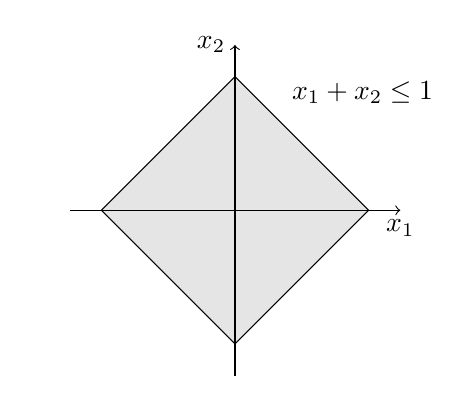
\begin{tikzpicture}[scale=0.6]
\draw[rotate around={45:(0,0)}, fill=black!10] (-2,-2) rectangle(2,2);
  \draw[->] (-3.5,0) -- (3.5,0) node[below] {$x_1$};
  \draw[->] (0,-3.5) -- (0,3.5) node[left] {$x_2$};
\draw[] (2.7,2.5) node {$\abs{x_1}+\abs{x_2}\leq 1$};
\draw[color=white] (-2.7,2.5) node {$\abs{x_1}+\abs{x_2}\leq 1$};
\end{tikzpicture}
\end{center}
$\norm{x}_{2} = \sqrt{\sum{x_{i}^{2}}} \leq 1$
\begin{center}
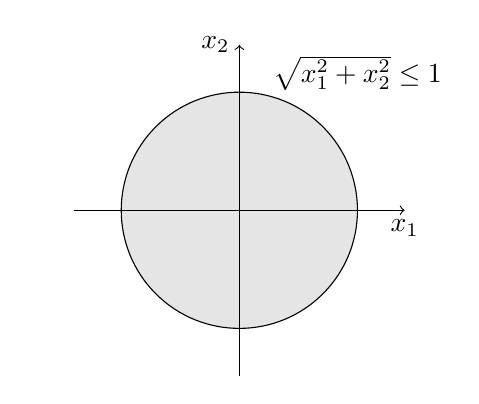
\begin{tikzpicture}[scale=0.6]
\draw[rotate around={45:(0,0)}, fill=black!10] (0,0) circle(2.5);
  \draw[->] (-3.5,0) -- (3.5,0) node[below] {$x_1$};
  \draw[->] (0,-3.5) -- (0,3.5) node[left] {$x_2$};
\draw[] (2.5,2.9) node {$\sqrt{x_1^2+x_2^2}\leq 1$};
\draw[color=white] (-2.5,2.9) node {$\sqrt{x_1^2+x_2^2}\leq 1$};
\end{tikzpicture}
\end{center}
$\mathop {\max }\limits_i \left\{ {\left| {{x_i}} \right|} \right\}=\norm{x}_{\infty} \leq 1$
\begin{center}
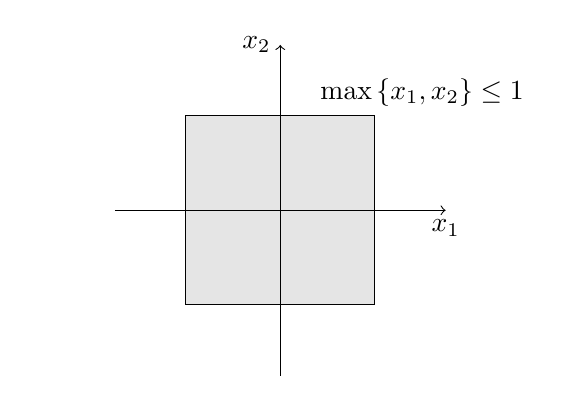
\begin{tikzpicture}[scale=0.6]
\draw[fill=black!10] (-2,-2) rectangle(2,2);
  \draw[->] (-3.5,0) -- (3.5,0) node[below] {$x_1$};
  \draw[->] (0,-3.5) -- (0,3.5) node[left] {$x_2$};
\draw[] (3,2.5) node {$\max\left\{\abs{x_1},\abs{x_2}\right\}\leq 1$};
\draw[color=white] (-3,2.5) node {$\max\left\{\abs{x_1},\abs{x_2}\right\}\leq 1$};
\end{tikzpicture}
\end{center}
\begin{definition}{4.15}
Zwei Normen $\norm{.}^{(1)}, \norm{.}^{(2)}$ auf $\R^{d}$ heissen \emph{äquivalent}, falls es $c_{1}, c_{2} > 0$ gibt, mit \[ c_{1}\norm{x}^{(1)}\leq\norm{x}^{(2)} \leq c_{2}\norm{x}^{(1)} \quad \forall x \in \R^{d} \]
\end{definition}
\noindent\textbf{Bemerkung}: Sei $C=\max{\{ C_{2}, \frac{1}{C_{1}}\}}$, dann gilt $(\frac{1}{C})\norm{x}^{(1)}\leq\norm{x}^{(2)} \leq C\norm{x}^{(1)}$
\subsubsection*{Beispiel}
Die Normen $\norm{.}_{p} \quad 1\leq p\leq\infty$ sind wegen $(\ast)$ äquivalent.
\subsubsection*{Bemerkung 4.16}
Äquivalente Normen definieren dieselben ``offenen Mengen'' via Distanzfunktion.
\subsubsection*{Beweis}
\todo{marked as skip? p152 week 9 sem1}Für die Normkugeln \[ B_{r}^{(1)}(x_{0})\defeq \{ x:\norm{x-x_{0}}^{(1)}<r\} \] gilt mit $c_{1}\norm{x}^{1}\leq\norm{x}^{2}\leq c_{2}\norm{x}^{1}$ \[ B_{rc_{1}}^{(1)}(x_{0}) \subset B_{r}^{(2)}(x_{0}) \subset B_{c_{2}r}(x_{0})\]
$\implies x_{0} \in \Omega$ innerer Punkt von $\Omega$ bezüglich $\norm{.}^{2} \iff x_{0}\in\Omega$ innerer Punkt von $\Omega$ bezüglich $\norm{.}^{1}$ \\

\noindent Auf $\R^{d}$ haben wir
\subsubsection*{Satz 4.17}
Je zwei Normen auf $\R^{d}$ sind äquivalent.
\subsubsection*{Beweis}
Es genügt zu zeigen, dass eine beliebige Norm $\norm{.}$ zu $\norm{.}_{2}$ äquivalent ist. \\
Seien $x=\sum{x_{i}e_{i}}$, $y=\sum{y_{i}e_{i}}$.
Dann ist
\begin{align*} \norm{x-y} = \norm{\sum_{i=1}^{d}{(x_{i}-y_{i})e_{i}}} \leq \sum_{i=1}^{d}{\abs{x_{i}-y_{i}}\norm{e_{i}}} &\leq \norm{x-y}\underbrace{\sum^{d}_{i=1}{\norm{e_{i}}}}_{\defeq C} \\
 &\underset{(\ast)}{\leq} C' \norm{x-y}_{2}\end{align*}
\todo{Layout imperfect, but hard to make better.. p153 week9 sem1}
\begin{align*}\text{Also folgt, dass } \R^{d}&\to \R \\ x &\mapsto \norm{x}\text{ stetig ist.}\end{align*}
Da $S^{d-1} = \{ x\in\R^{d}:\norm{x}_{2}=1\}$ kompakt ist, folgt dass es $c_{+}, c_{-}\in S^{d-1}$ gibt, mit ${k_{-}\defeq\norm{c_{-}}}\leq\norm{x}\leq{\norm{c_{+}}\defeq k_{+}} \: \forall x\in S^{d-1}$. Da $c_{0}\neq 0$ folgt $k_{-}>0$. \\
Sei $x\neq0$allgemein ($C_{-}\in S^{d-1}$), dann ist $y\defeq\frac{x}{\norm{x}_{2}}\in S^{d-1}$ also $k_{-}\leq \norm{\frac{x}{\norm{x}_{2}}}<k_{+}$, woraus \[ k_{-}\norm{x}_{2}\leq\norm{x}\leq k_{+}\norm{x}_{2}\] folgt.

\section{$\varepsilon -\delta$ Kriterium für Stetigkeit}
\todo{4.5 in source notes. what to do?}
Wir haben das folgende Kriterium für Stetigkeit an der Stelle $x_{0}$:

\subsubsection*{Satz 4.18}
Sei $f:\Omega\to\R^{n}$, $\Omega\subset\R^{d}$ eine Abbildung, $x_{0} \in\Omega$. Folgende Eigenschaften sind äquivalent:
\begin{enumerate}
\item $f$ ist stetig an der Stelle $x_{0}$. \\ D.h. für jede gegen $x_{0}$ konvergierende Folge $(x_{n})\subset\Omega$ konvergiert die Folge $f(x_{n})$ gegen $f(x_{0})$.
\item Für jedes $\varepsilon>0$ gibt es $\delta>0$ so dass für alle $x\in\Omega$ mit $\abs{x-x_{0}}<\delta$ gilt:\[ \abs{\delta(x)-\delta(x_{0})}<\varepsilon \]
\[ \forall\varepsilon>0\;\exists\delta>0: \forall x\in\Omega,\norm{x-x_{0}}<\delta \implies \norm{\delta(x)-\delta(x_{0})}<\varepsilon\]
\end{enumerate}

\begin{beweis}{4.18}
\begin{enumerate}[align=left]
\item[$(1)\Rightarrow (2)$] (Indirekt)\\
Wir nehmen also an, dass (2) nicht gilt, d.h. es gibt $\varepsilon>0$ so dass für jedes $\delta >0$ einem punkt $x_\delta$ gibt mit 
\[\left\| {{x_\delta } - {x_0}} \right\| < \delta {\text{ und }}\left\| {f\left( {{x_\delta }} \right) - f\left( {{x_0}} \right)} \right\| > \varepsilon \]
\todo[inline]{Start of big bracket}
\begin{align*}
&\neg \left( {\forall \varepsilon  > 0,\exists \delta  > 0,\forall x \in \Omega :\left| {x - {x_0}} \right| < \delta  \Rightarrow \left| {f\left( x \right) - f\left( {{x_0}} \right)} \right| < \varepsilon } \right)\\
 &= \left( {\exists \varepsilon  > 0,\forall \delta  > 0,\exists x \in \Omega :\left| {x - {x_0}} \right| < \delta {\text{ }}\not  \Rightarrow {\text{ }}\left| {f\left( x \right) - f\left( {{x_0}} \right)} \right| < \varepsilon } \right)
\end{align*}
d.h.
\[\exists \varepsilon  > 0,\forall \delta  > 0,\exists {x_\delta } \in \Omega :\left| {{x_\delta } - {x_0}} \right| < \delta {\text{  und  }}\left| {f\left( x \right) - f\left( {{x_0}} \right)} \right| > \varepsilon \]
\todo[inline]{end of big bracket}
Sei $\varepsilon>0$. Wir wählen jetzt $\delta_n=\frac{1}{n}$, dann gibt es $x_n:=\left(x_{\delta_n}\right)_{n\in\N}$, eine Folge in $\Omega$, mit $\lim x_n=x_0$. Aber die Folge $\left( f\left( x_n\right)\right)$ kann offensichtlich nicht gegen $f\left( x_0\right)$ konvergieren (Da $\left| {f\left( {{x_n}} \right) - f\left( {{x_0}} \right)} \right| > \varepsilon $), d.h. $f$ ist nicht stetig in $x_0$ 
\item[$(2)\Rightarrow (1)$] Sei $\left( x_n\right)_{n\geq 1}$ eine Folge in $\Omega$ mit Grenzwert $x_0$. Wir möchten zeigen dass $f\left( {{x_n}} \right) \to f\left( {{x_0}} \right)$. Sei $\varepsilon>0$, nach (2) sei $\delta_{\varepsilon}>0$ so dass $\forall x\in\Omega$ mit 
\[\left| {x - {x_0}} \right| < {\delta _\varepsilon } \Rightarrow \left| {f\left( x \right) - f\left( {{x_0}} \right)} \right| < \varepsilon \]
Da $\mathop {\lim }\limits_{n \to \infty } {x_n} = {x_0}$, gibt es $N\geq 1$ so dass 
\[\left\| {{x_n} - {x_0}} \right\| < \delta\hspace{5mm} \forall n \ge {N_\delta }\]
(Hier hängt $N$ von $\delta$, und also im Endeffekt von $\varepsilon$ ab). Aus (2) folgt
\[\left\| {f\left( {{x_n}} \right) - f\left( {{x_0}} \right)} \right\| < \varepsilon \hspace{5mm}\forall n \ge {N_\delta }\]
Dies zeigt $\lim f\left( {{x_n}} \right) = f\left( {{x_0}} \right)$
\end{enumerate}
\end{beweis}

\subsubsection*{Beispiel}
\begin{enumerate}
\item $f:\R\to\R$, $f(x)=3x+8$. Dann $f$ ist stetig auf $\R$. Sei $\varepsilon>0$, sei $x_0\in\R$
\[\left| {f\left( x \right) - f\left( {{x_0}} \right)} \right| = \left| {\left( {3x + 8} \right) - \left( {3{x_0} + 8} \right)} \right| = 3\left| {\left( {x - {x_0}} \right)} \right|\hspace{5mm}\forall x \in \R\]
Sei $\varepsilon>0$. Wenn wir $\delta=\frac{\varepsilon}{3}$ wählen, dann 
\[ \text{CAN'T READ}, \left| {x - {x_0}} \right| < {\delta _\varepsilon } = \frac{\varepsilon }{3} \Rightarrow \left| {f\left( x \right) - f\left( {{x_0}} \right)} \right| < \varepsilon \]
In diesem Beispiel $\delta$ hängt nur von $\varepsilon$ ab. Nächste Beispiel zeigt dass $\delta$ nicht nur von $\varepsilon$, sondern auch von $x_0$ abhängen kann.
\item \begin{align*}
f:\left( 0,\infty\right)\to&\left( 0,\infty\right)\\
x\to&\frac{1}{x}
\end{align*}
ist stetig auf $\left( 0,\infty\right)$. Sei $x_0\in\left( 0,\infty\right)$
\[\left| {f\left( x \right) - f\left( {{x_0}} \right)} \right| = \left| {\frac{1}{x} - \frac{1}{{{x_0}}}} \right| = \left| {\frac{{{x_0} - x}}{{x \cdot {x_0}}}} \right|\]
\[\left| {x - {x_0}} \right| < \delta  \Rightarrow  - \delta  < x - {x_0} < \delta  \Rightarrow x > {x_0} - \delta \]
\[\left| {f\left( x \right) - f\left( {{x_0}} \right)} \right| = \frac{{\left| {{x_0} - x} \right|}}{{\left| x \right|\left| {{x_0}} \right|}} < \frac{{\left| {x - {x_0}} \right|}}{{\left| {{x_0}} \right|\left| {{x_0} - \delta } \right|}}\]
Sei $\delta<\frac{x_0}{2}$, dann folgt 
\[\delta  < \frac{{{x_0}}}{2} \Rightarrow {x_0} - \delta  > {x_0} - \frac{{{x_0}}}{2} > \frac{{{x_0}}}{2}\]
\[\left| {f\left( x \right) - f\left( {{x_0}} \right)} \right| < \frac{{\left| {{x_0} - x} \right|}}{{\left| x \right|\left| {{x_0} - \delta } \right|}} \le \frac{{\left| {x - {x_0}} \right| \cdot 2}}{{{{\left| {{x_0}} \right|}^2}}} \le \frac{{2\delta }}{{\left| {{x_0}} \right|}}\]
Sei 
\[{\delta _{\varepsilon ;{x_0}}} = \min \left\{ {\frac{{{x_0}}}{2},\frac{{\varepsilon {{\left| {{x_0}} \right|}^2}}}{2}} \right\}\]
Dann
\[\left| {f\left( x \right) - f\left( {{x_0}} \right)} \right| < \frac{{\varepsilon {{\left| {{x_0}} \right|}^2}}}{2} \cdot \frac{2}{{{{\left| {{x_0}} \right|}^2}}} = \varepsilon \]
\end{enumerate}

\section{Zwischenwertsatz}
\subsubsection*{Satz 4.19}
Seien $a<b$ in $\R$ und $f:\lbrack a,b\rbrack\to\R$ eine Stetige Funktion, mit $f(a)\leq f\left( b\right)$ (oder $f(a)\geq f\left( b\right)$). Dann gibt es zu jedem $y\in\left[ f(a),f\left( b\right)\right]$ ein $x\in\left[ a,b\right]$ mit $f(x)=y$

\begin{beweis}{}
Idee ist einfach. Wir benutzen ein Approximationsverfahren (In diesem Fall Bisektionsverfahren). Wir definieren zwei Monotone Folgen
\[ a=a_1\leq a_2\leq\dots\leq b_2\leq b_1=b\]
mit $a_n\nearrow$, $b_n\searrow$, $\lim a_n=\lim b_n=c$ und 
\[ f\left( a_n\right)<y\leq f\left( b_n\right)\]
Dann aus stetigkeit von $f$, folgt dass 
\[ \lim f\left( a_n\right)=\lim f\left( b_n\right)=f(c)=y\]
\begin{multicols}{2}
\begin{center}
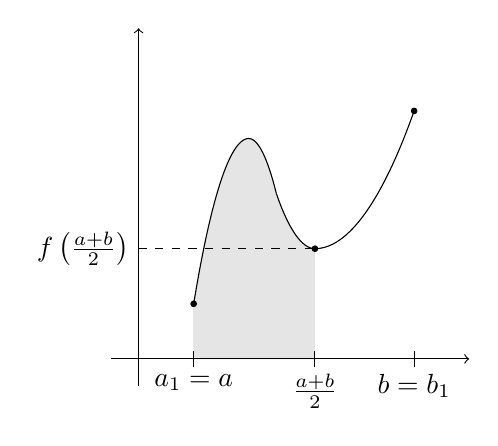
\begin{tikzpicture}[scale=0.7]
\shade[top color=black!10,bottom color=black!10] 
      (1,1) parabola bend (2,4)(2.5,3)
(2.5,3) parabola bend (3.2,2)(3.2,0) ;
\draw[color=black!10,fill=black!10] (1,0) rectangle (3.18,1)
(1,1) -- (2.5,3) -- (3.2,0)-- (1,1);
\draw[->](-0.5,0) -- (6,0);
\draw[->](0,-0.5) -- (0,6);
\draw (1,1) parabola bend (2,4) (2.5,3);
\draw (2.5,3) parabola bend (3.2,2) (5,4.5); 
\draw[fill=black] (1,1) circle (0.05);
\draw[fill=black] (5,4.5) circle (0.05);
\draw[fill=black] (3.2,2) circle (0.05);
\draw[](1,-0.15) -- (1,0.15) node[anchor=north,yshift=-5] {$a_1=a$};
\draw[](3.2,-0.15) -- (3.2,0.15) node[anchor=north,yshift=-5] {$\frac{a+b}{2}$};
\draw[](5,-0.15) -- (5,0.15) node[anchor=north,yshift=-5] {$b=b_1$};
\draw[dashed](0,2) -- (3.25,2);
\draw (0,2) node[anchor=east] {$f\left(\frac{a+b}{2}\right)$};
\end{tikzpicture}
\end{center}
\vspace{-1.5mm}
\setlength{\leftskip}{1.2cm}
\centerline{\hspace*{6mm}\underline{Fall 1:}}\vspace{2mm}
Falls $f\left(\frac{a+b}{2}\right)\geq y$, setzen wir:
\begin{align*}
a_2&=a\\
b_2&=\frac{a+b}{2}
\end{align*}
\setlength{\leftskip}{0cm}
\columnbreak
\begin{center}
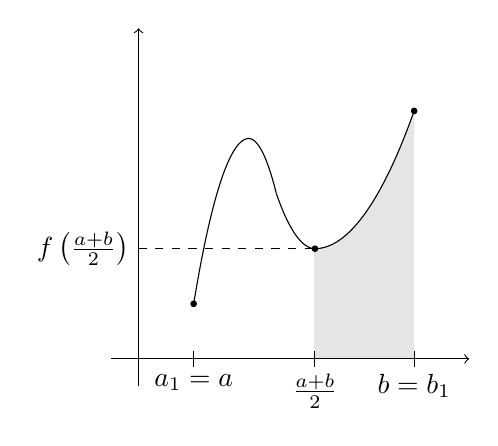
\begin{tikzpicture}[scale=0.7]
\shade[top color=black!10,bottom color=black!10] 
      (3.2,2) parabola bend (3.2,2) (5,4.5) |- (3.2,2);
\draw[color=black!10,fill=black!10] (3.2,0) rectangle (4.99,2);
\draw[->](-0.5,0) -- (6,0);
\draw[->](0,-0.5) -- (0,6);
\draw (1,1) parabola bend (2,4) (2.5,3);
\draw (2.5,3) parabola bend (3.2,2) (5,4.5); 
\draw[fill=black] (1,1) circle (0.05);
\draw[fill=black] (5,4.5) circle (0.05);
\draw[fill=black] (3.2,2) circle (0.05);
\draw[](1,-0.15) -- (1,0.15) node[anchor=north,yshift=-5] {$a_1=a$};
\draw[](3.2,-0.15) -- (3.2,0.15) node[anchor=north,yshift=-5] {$\frac{a+b}{2}$};
\draw[](5,-0.15) -- (5,0.15) node[anchor=north,yshift=-5] {$b=b_1$};
\draw[dashed](0,2) -- (3.25,2);
\draw (0,2) node[anchor=east] {$f\left(\frac{a+b}{2}\right)$};
\end{tikzpicture}
\end{center}
\setlength{\leftskip}{1.2cm}
\centerline{\hspace*{6mm}\underline{Fall 2:}}\vspace{2mm}
Falls $f\left(\frac{a+b}{2}\right)< y$, setzen wir:
\begin{align*}
a_2&=\frac{a+b}{2}\\
b_2&=b_1
\end{align*}
\setlength{\leftskip}{0cm}
\end{multicols}
Auf jedem Fall gibt
\begin{enumerate}
\item $a_1\leq a_2 < b_2 \leq b_1$
\item $\left( b_2-a_2\right)=\frac{1}{2}\left( b_1-a_1\right)$
\item $f\left( a_2\right) < y \leq f\left( b_2\right)$
\end{enumerate}
Wir iterieren jetzt dieses Verfahren. Wir nehmen an, dass wir Folgen definiert haben nach $(k-1)-$Schnitten 
\begin{enumerate}
\item $a_1\leq a_2\leq a_3\dots\leq a_k < b_k\leq b_{k-1}\dots\leq b_1$
\item $\left( {{b_k} - {a_k}} \right) = \frac{1}{{{2^{k - 1}}}}\left( {{b_1} - {a_1}} \right)$
\item $f\left( a_k\right) < y \leq f\left( b_k\right)$
\end{enumerate}
Nun unterscheiden wir wieder zwei Fälle\\

\noindent\underline{Fall 1:}
\[f\left( {\frac{{{a_k} + {b_k}}}{2}} \right) \ge y\] dann definieren wir $a_{k+1}=a_k$ und $b_{k+1}=\frac{a_k+b_k}{2}$\\

\noindent\underline{Fall 2:}
\[f\left( {\frac{{{a_k} + {b_k}}}{2}} \right) < y\]
dann definieren wir $a_{k+1}=\frac{a_k+b_k}{2}$ und $b_{k+1}=b_k$. Dann ist immer
\begin{enumerate}
\item $a_k\leq a_{k+1}<b_{k+1}\leq b_k$
\item ${b_{k + 1}} - {a_{k + 1}} = \frac{1}{2}\left( {{b_k} - {a_k}} \right) = \frac{1}{{{2^k}}}\left| {{b_1} - {a_1}} \right|$
\item $f\left( a_{k+1}\right) < y \leq f\left( b_{k+1}\right)$
\end{enumerate}
Nach dem Prinzip der Vollständigen Induktion erhalten wir zwei folgen $\left( a_n\right)_{n\geq 1}$, $\left( b_n\right)_{n\geq 1}$ die den Eigenschaften 1., 2. und 3. erfüllen. $\left( a_n\right)$, $\left( b_n\right)$ sind monotone und beschränkt $\Rightarrow$ gibt es 
\[\overline{a}=\lim a_k\leq\overline{b}=\lim b_k \]
Wegen 2.
\[\lim \left| {{a_k} - {b_k}} \right| = \lim \left| {\frac{{{b_1} - {a_1}}}{{{2^k}}}} \right| = 0\]
d.h. $\lim a_k=\lim b_k$. Sei $c\in\lbrack a,b\rbrack$ dieser Wert. Aus stetigkeit von $f$ folgt 
\[f\left( c \right) = \lim f\left( {{a_n}} \right) = \lim f\left( {{b_n}} \right)\]
Aus 3. folgt 
\begin{align*}
f\left( {{a_n}} \right) < y &\Rightarrow f\left( c \right) \le y\\
g \le f\left( {{b_n}} \right) &\Rightarrow y \le f\left( c \right)
\end{align*}
also $f(c)=y$.
\end{beweis}

\subsubsection*{Korollar 4.20}
\begin{enumerate}
\item Sei
\[p\left( x \right) = {a_n}{x^n} + {a_{n - 1}}{x^{n - 1}} +  \ldots  + {a_0}\]
ein polynome mit reellen Koeffizienten so dass $a_n\not=0$ und $n$ ungerade ist. Dann besitzt $p$ mindestens eine reelle Nullstelle.
\begin{beweis}{}
Sei 
\begin{align*}
q(x) &= \frac{{p(x)}}{{{a_n}}}\\
 &= {x^n} + \frac{{{a_{n - 1}}}}{{{a_n}}} \cdot {x^{n - 1}} +  \ldots  + \frac{{{a_0}}}{{{a_n}}}\\
 &= {x^n}\left[ {1 + \frac{{{a_{n - 1}}}}{{{a_n}}} \cdot \frac{1}{x} +  \ldots  + \frac{{{a_0}}}{{{a_n}}} \cdot \frac{1}{{{x^n}}}} \right]
\end{align*}
Dann
\[\mathop {\lim }\limits_{x \to \infty } \frac{1}{{{x^5}}} = 0\]
Folgt insbesondere dass es $c>0$ gibt so dass für $\abs{x}\geq c$ 
\[1 + \frac{{{a_{n - 1}}}}{{{a_n}}} \cdot \frac{1}{x} +  \ldots  + \frac{{{a_0}}}{{{a_n}}} \cdot \frac{1}{{{x^n}}} \ge \frac{1}{2}\]
Folglich ist:
\begin{align*}
q(c) &\ge {c^n}\frac{1}{2} > 0\\
q( - c) &\le  - {c^n}\frac{1}{2} < 0\tag{\text{$n=$ ungerade}}
\end{align*}
Also gibt $x_0\in\lbrack -c,c\rbrack$ mit $q\left( x_0\right)=0$
\end{beweis}
\item Eine reelle $3\times 3$ Matrix besitzt immer einen reellen Eigenwert.
\end{enumerate}

\subsubsection*{Satz 4.21}
Sei $f:\lbrack a,b\rbrack\to\R$ stetig, streng monoton Wachsend (d.h. $x<y=f(x)<f\left( y\right)$). Dann ist 
\[\Bild\left( f\right)=\lbrack c,d\rbrack=\left[ f\left( a\right), f\left( b\right)\right]\]
$f:\lbrack a,b\rbrack\to\lbrack c,d\rbrack$ is bijektiv und $f^{-1}:\lbrack c,d\rbrack\to\lbrack a,b\rbrack$ ist stetig

\begin{beweis}{}
\begin{enumerate}
\item $f$ streng monoton wachsend, d.h. Falls $x\not=y$, dann ist $f\left( x\right)\not=f\left( y\right)\Rightarrow f$ Injektive.\\

Zwischenwertsatz $\Rightarrow f$ surjektive. $c=f(a)<f(b)=d$, Sei $y\in\lbrack c,d\rbrack$, ZWS $\Rightarrow\exists x\in\left( a,b\right)$ mit $f(x)=y\Rightarrow$ ist bijektive
\item $f^{-1}$ ist stetig: Sei $y\in\lbrack c,d\rbrack$ und sei $\left( y_0\right)\in\lbrack c,d\rbrack$ eine folge mit $\lim y_n=y_0$. $f$ bijektive, $\exists x_n$, $x_0=f^{-1}\left( y_0\right)$, $\left( x_n\right)$ beschränkt. Sei $f^{-1}\left( y_{l(n)}\right)$ eine beliebige konvergente Teilfolge und $x$ deren Grenzwert 
\[ \lim f^{-1}\left( y_{l(n)}\right)=x\]
\[ f\text{ stetig }\Rightarrow\lim f\left( f^{-1}\left( y_{l(n)}\right)\right) = f\left( f^{-1}\left( y_{l(n)}\right)\right)= f(x) \]
aber 
\[\lim f\left( {{f^{ - 1}}\left( {{y_{l(n)}}} \right)} \right) = \lim {y_{l(n)}}\]
\begin{enumerate}
\item[$\Rightarrow$] $\lim {y_{l(n)}}=f(x)$, $y_n$ ist aber auch konvergent
\item[$\Rightarrow$] $\lim {y_{(n)}}=f(x)$, aber $\lim y_n=y_0$
\item[$\Rightarrow$] $y_0=f(x)\Rightarrow x=f^{-1}\left( y_0\right)=x_0$
\item[$\Rightarrow$] Jede Teilfolge von $\left( x_0\right)$ hat desselben Häufungspunkt $x_0$.
\item[$\Rightarrow$] $\lim\sup x_n=x_0=\lim\inf x_n$, also $\lim {f^{ - 1}}\left( {{y_n}} \right) = \lim {x_n} = {x_0} = {f^{ - 1}}\left( {{y_0}} \right)\Rightarrow f$ stetig 
\end{enumerate}
\end{enumerate}
\end{beweis}

\subsubsection*{Korollar 4.22}
Sei $f:\left( a,b\right)\to\R$ stetig und streng monoton wachsend mit monotonen Limes
\[ - \infty  < c: = \mathop {\lim }\limits_{x \downarrow a} f\left( x \right) < \mathop {\lim }\limits_{x \uparrow b} f\left( x \right) = :d < \infty \]
dann ist $f:\left( a,b\right)\to\left( c,d\right)$ bijektive und $f^{-1}$ ist stetig.

\subsubsection*{Korollar 4.22}
Sei $n\in\N$. Die Potenzfunktion $f(x)=x^n$ ist auf ganz $\R$ stetig. Sie ist auf $\left( 0,\infty\right)$ streng monoton wachsend mit Bild $\left( 0,\infty\right)$. Die Umkehrfunktion 
\begin{align*}
\left( 0,\infty\right)&\to\left( 0,\infty\right)\\
x&\to\sqrt[n]{x}\text{ ist stetig}
\end{align*}

\begin{beweis}{}
\[{y^n} - {x^n} = \left( {y - x} \right)\underbrace {\left( {{y^{n - 1}} + {y^{n - 2}}x +  \ldots {x^{n - 1}}} \right)}_{ > 0}\]
Für $0<x,y<\infty$, ${y^{n - 1}} + {y^{n - 2}}x +  \ldots {x^{n - 1}}>0$.
Also folgt $x<y\Rightarrow x^n<y^n$, d.h. $f$ streng monoton wachsend
\end{beweis}

\subsubsection*{Satz 4.23}
Die Funktion $\exp:\R\to\R$ ist stetig, streng monotone wachsend mit 
\[ \Bild\left( \exp\right)=\exp\left( \R\right)=\left( 0,\infty\right)\]

\begin{definition}{4.24}
Die Umkehrfunktion von $\exp:\R\to\left( 0,\infty\right)$ wird mit $\log:\left( 0,\infty\right)\to\R$ bezeichnet
\end{definition}
Dann

\subsubsection*{Korollar 4.25}
$\log:\left( 0,\infty\right)\to\R$ hat folgende Eigenschaften
\begin{enumerate}
\item Sie ist strikt monoton wachsend und stetig
\item $\log(1)=0$
\item $\log\left( x\cdot y\right)=\log(x)+\log\left( y\right)$
\end{enumerate}

\begin{beweis}{Satz 4.23}
\[\exp \left( x \right) = 1 + x + \frac{{{x^2}}}{{2!}} +  \ldots \]
ist absolut konvergent auf ganz $\R$
\begin{enumerate}
\item \[\exp \left( x \right) = \exp \left( {\frac{x}{2} + \frac{x}{2}} \right) = {\left( {\exp \left( {\frac{x}{2}} \right)} \right)^2} \ge 0\]
\item Falls $x\geq 0$, ist \[\exp \left( x \right) > 1 > 0\hspace{5mm}\left( {\exp \left( x \right) = 1 \Leftrightarrow x = 0} \right)\]
\item Wegen \[\exp \left( x \right) = \frac{1}{{\exp \left( { - x} \right)}}\not  = 0\] \[\exp \left( x \right) > 0\hspace{5mm}\forall x \in \R\] d.h. \[\exp\left( \R\right)\subset\left( 0,\infty\right)\]
\item \[\exp \left( y \right) - \exp \left( x \right) = \exp \left( x \right)\left[ {\exp \left( {y - x} \right) - 1} \right]\]
Falls $x<y$, so ist $\exp\left(y-x\right)>1$ und somit $\exp\left(y\right)>\exp\left(x\right)$ (da $\exp\left(x\right)>0$), d.h. $\exp$ ist streng monoton Wachsend
\item Zur stetigkeit: Sei $x=x_0+h$, $0<h<1$
\[\exp \left( x \right) - \exp \left( {{x_0}} \right) = \exp \left( {{x_0}} \right)\left( {\exp \left( h \right) - 1} \right)\]
da 
\[\left| {\exp \left( h \right) - 1} \right| = \mathop {\left| {\sum\limits_{k = 1}^\infty  {\frac{{{h^k}}}{{k!}}} } \right|}\limits^{ \to 0}  \le \mathop {\left| {\sum\limits_{k = 1}^\infty  {\left| {{h^k}} \right|} } \right|}\limits^{h \to 0}  = \frac{{\left| h \right|}}{{1 - \left| h \right|}} \to 0\]
Also für $x=x_0+h\to x_0$, $\exp\left( x \right)-\left( x_0 \right)\to 0$ und die Funktion $\exp$ ist stetig
\[\exp \left( x \right) \to \infty \left( {x \to \infty } \right){\text{ und }}\exp \left( x \right) \to 0\left( {x \to  - \infty } \right)\]
\end{enumerate}
\todo[inline]{do 3 and 4 belong together?? in your notes you gave number 3 to two different ones, page 166 bottom}
\end{beweis}

\begin{align*}
\exp\left( \log(x)\right)&=x\\
\exp\left( \log\left(x\right)+\log\left(y\right)\right)&=\exp\left( \log\left(x\right)\right)\cdot\exp\left( \log\left(x\right)\right)\\
&=xy
\end{align*}
\[ \Rightarrow\boxed{\log\left( x\right)+\log\left( y\right)=\log\left( xy\right)}\]

\section{Gleichmässig Stetigkeit}
Sei $f:\Omega\to\R$ eine stetige funktion auf $\Omega$, d.h. 
\[\forall {x_0} \in \Omega ,\forall \varepsilon  > 0,\exists \delta  > 0,\forall x \in \R :\left| {x - {x_0}} \right| < \delta  \Rightarrow \left| {f\left( x \right) - f\left( {{x_0}} \right)} \right| < \varepsilon \]
\todo[inline]{Begin big rounded parenthesis}
$f$ ist nicht stetig auf $\Omega\Leftrightarrow\exists x_0\in\Omega,\exists\varepsilon>0,\forall>0,\exists\in\Omega:\abs{x-x_0}<\delta\text{ und }\abs{f\left( x\right)-f\left( x_0\right)}\geq\varepsilon$
\todo[inline]{End big rounded parenthesis}

\begin{definition}{4.24}
\underline{Gleichmässig stetig:} \vspace{2mm}\\
$f:\Omega\to\R^n$ heisst gleichmässig stetig falls für jede $\varepsilon>0$, ein $\delta>0$ gibt so dass $\forall x,x_0\in\Omega$
\[\left\| {x - {x_0}} \right\| < \delta  \Rightarrow \left| {f\left( x \right) - f\left( {{x_0}} \right)} \right| < \varepsilon \]
\underline{Stetig:} \vspace{2mm}\\
$\forall x_0\in\omega$, $\forall \varepsilon>0$, $\exists\delta_{x_0,\varepsilon}>0$, $\forall x\in\Omega$:
\[\left| {x - {x_0}} \right| < \delta  \Rightarrow \left| {f\left( x \right) - f\left( {{x_0}} \right)} \right| < \varepsilon \]
\underline{Gleich stetig:} \vspace{2mm}\\
$\forall \varepsilon>0$, $\exists\delta_{\varepsilon}>0$, $\forall x,x_0\in\Omega$:
\[\left| {x - {x_0}} \right| < \delta  \Rightarrow \left| {f\left( x \right) - f\left( {{x_0}} \right)} \right| < \varepsilon \]
Stetig: $\delta$ ist abhängig von $\varepsilon$ und $x_0$\\
gleich. stetig:$\delta$ ist abhängig von $\varepsilon$, aber unabhängig con $x_0$
\end{definition}

\subsubsection*{Beispiel 4.25}
\begin{enumerate}[I)]
\item $\exp:\R\to\R$ ist nicht gleichmässig stetig \[\abs{\exp(x)-\exp\left( x_0\right)}=\abs{\exp\left( x-x_0\right)-1}\exp\left( x_0\right)\]
Falls $x-x_0=\pm\delta$, $\delta\not=0$ und $x_0\to\infty$ dann
\[\abs{\exp(x)-\exp\left( x_0\right)}\to\infty\]
\item \begin{align*}
f(x):\R&\to\R\\
x&\to 2x+5
\end{align*}
Dann ist $f$ gleichmässigstetig
\begin{beweis}{}
Sei $\varepsilon>0$, $x_0,x\in\R$. Dann \[\left| {f\left( x \right) - f\left( {{x_0}} \right)} \right| = \left| {2x + 5 - 2{x_0} + 5} \right| = 2\left| {x - {x_0}} \right|\]
$\Rightarrow$ Wenn wir $\delta=\frac{\varepsilon}{2}$ wählen, dann \[\left| {x - {x_0}} \right| < \frac{\varepsilon }{2} \Rightarrow \left| {f\left( x \right) - f\left( {{x_0}} \right)} \right| < \varepsilon \] 
\end{beweis}
\item \begin{align*}
f:\Omega&\to\Omega\hspace{5mm}\Omega=\left( 0,\infty\right)\\
x&\to x^2
\end{align*}
$f$ ist stetig aber nicht gleichmässig stetig. 
\begin{enumerate}[i)]
\item $f$ stetig: Sei $x_0\in\R$, $\varepsilon>0$\[\left| {f\left( x \right) - f\left( {{x_0}} \right)} \right| = \left| {{x^2} - x_0^2} \right| = \left| {\left( {x - {x_0}} \right)\left( {x + {x_0}} \right)} \right|\] Sei $\abs{x-x_0}<\varepsilon<1$. Dann, $x<x_0+1:=a$. Dann $x,x_0+1<a$
\[\left| {{x^2} - x_0^2} \right| = \left| {x - {x_0}} \right|\left| {x + {x_0}} \right| < 2a\left| {x - {x_0}} \right|\]
Wenn wir $\delta=\min\left(1,\frac{\varepsilon}{2a}\right)$ wählen dann \[\left| {x - x_0^2} \right| < 2a\left| {x - {x_a}} \right| \le \varepsilon \]
\subsubsection*{Bemerkung}
$f$ ist abhängig von $\varepsilon$, und $a$ ist $x_0+1$, abhängig von $x_0$.
\item $f$ ist nicht gleichmässig stetig, d.h. \[\exists \varepsilon  > 0, \forall\delta>0, \exists x_0\in\Omega, \exists x\in\Omega:\abs{x-x_0}<\delta \text{ und }\abs{x^2-x_0^2}\geq \varepsilon\]
Sei $\varepsilon=1$, $\delta>0$, $x_0=\frac{1}{\delta}$ und $x=x_0+\frac{\delta}{2}$. Dann $\abs{x-x_0}<\frac{\delta}{2}<\delta$ aber \[\left| {{x^2} - x_0^2} \right| = \left| {{{\left( {\frac{1}{\delta } + \frac{\delta }{2}} \right)}^2} - \frac{1}{{{\delta ^2}}}} \right| = 1 + \frac{{{\delta ^2}}}{4} > 1 = \varepsilon \]
\end{enumerate}
\item \begin{align*}
f:\Omega&\to\Omega\hspace{5mm}\Omega=\lbrack 0,4\rbrack\\
x&\to x^2
\end{align*}
Dann ist $f$ gleichmässig stetig
\begin{beweis}{}
Sei $\varepsilon>0$ gegeben. Sei $x_0,x\in\Omega=\lbrack 0,4\rbrack$, $0\leq x,x_0\leq 4\Rightarrow 0\leq x+x_0\leq 8$
\begin{align*}
\left| {x - {x_0}} \right| < \delta  \Rightarrow \left| {f\left( x \right) - f\left( {{x_0}} \right)} \right| &= \left| {{x^2} - x_0^2} \right|\\
 &= \left| {x - {x_0}} \right|\left| {x + {x_0}} \right| \le \left( {4 + 4} \right)\delta 
\end{align*}
Sei $\delta=\frac{\varepsilon}{8}$, dann 
\[\left| {x - {x_0}} \right| < \delta  \Rightarrow \left| {f\left( x \right) - f\left( {{x_0}} \right)} \right| < \varepsilon \]
\end{beweis}
\item  \begin{align*}
f:\left( 0,\infty\right)&\to\left( 0,\infty\right)\\
x&\to \sqrt{x}
\end{align*}
ist gleichmässig stetig auf $\left( 0,\infty\right)$
\begin{beweis}{}
\todo[inline]{Ask for beweis! page 172 bottom}
\end{beweis}
\end{enumerate}

Wir haben gesehen dass 
 \begin{align*}
f:\left( 0,\infty\right)&\to\left( 0,\infty\right)\\
x&\to x^2
\end{align*}
nicht gleichmässig stetig ist, aber 
 \begin{align*}
f:\left[ 0,4\right]&\to\left[ 0,4\right]\\
x&\to x^2
\end{align*}
ist gleichmässig stetig. Was ist die Unterschied? $\lbrack 0,4\rbrack$ ist kompakt, $\left( 0,\infty\right)$ nicht

\subsubsection*{Satz 4.26}
Sei $K\subset\R^d$ kompakt und $f:K\to\R^n$ stetig. Dann ist $f$ gleichmässig stetig.

\begin{beweis}{(Indirekt)}
Sonst es gibt $\varepsilon>0$ so dass für jedes $\delta>0$ Punkte $x,y\in k$ gibt mit \[\left\| {x - y} \right\| < \delta \hspace{5mm}\left| {f\left( x \right) - f\left( y \right)} \right| > \varepsilon \]
Sei $\forall k\geq 1$, mit $\delta=\frac{1}{k}$, ein Paar $\left( x_k,y_k\right)$ gewählt so dass\[\left| {{x_k} - {y_k}} \right| < \frac{1}{k}{\text{ und }}\left| {f\left( {{x_k}} \right) - f\left( {{y_k}} \right)} \right| > \varepsilon \]
Da $k$ kompakt ist, gibt eine konvergente Teilfolge $x_{l(k)}\to z$. Aus $\abs{x_k-y_k}<\frac{1}{k}$ folgt dass $y_{l(k)}\to z$. Sei nun $k_0$ so dass 
\[\mathop {\left\| {f\left( {{x_{l\left( {{k_0}} \right)}}} \right) - f\left( z \right)} \right\|}\limits_{f{\text{ stetig}}} < \frac{\varepsilon }{2}\hspace{5mm}\forall k > {k_0}\]
Dann folgt $\forall k>k_0$:
\[\left\| {f\left( {{y_{l\left( {{k_0}} \right)}}} \right) - f\left( z \right)} \right\| \ge \left| {\underbrace {f\left( {{y_{l\left( k \right)}}} \right) - f\left( {{x_{l\left( k \right)}}} \right)}_{ > \varepsilon }} \right| - \left| {\underbrace {f\left( {{x_{l\left( k \right)}}} \right) - f\left( z \right)}_{ < \varepsilon /2}} \right| \ge \frac{\varepsilon }{2}\]
\end{beweis}

\section{Punktweise und gleichmässige Konvergenz}
Sei $\Omega\subset\R^d$, $f,f_k:\Omega\to\R^n$

\begin{definition}{4.28}
$\left( f_k\right)_{k\geq 1}$ konvergiert punktweise gegen $f$ falls $\forall x\in\Omega$ \[\mathop {\lim }\limits_{k \to \infty } {f_k}\left( x \right) = f\left( x \right)\]
$\forall x\in\Omega$, $\forall\varepsilon>0$, $\exists k_{\varepsilon,x}$ s.d. $\abs{f_k(x)-f(x)}<\varepsilon$, $\forall k>k_{\varepsilon,x}$. Es stellt sich die Frage ob $f$ stetig ist, falls alle $\left( f_k\right)_{k\geq 1}$ stetig sind
\end{definition}
\subsubsection*{Beispiel 4.30}
Sei $f_k:\lbrack 0,1\rbrack\to\R$, $f_k(x)=x^k$, $k\geq 1$. Dann gilt 
\begin{align*}
0 \le x < 1:&\mathop {\lim }\limits_{k \to \infty } {x^k} = 0\\
x = 1:&\mathop {\lim }\limits_{x \to \infty } {x^k} = 1
\end{align*}
Also konvergiert $\left( f_k\right)$ punktweise gegen 
\[f(x) = \left\{ {\begin{array}{*{20}{r}}
0&{0 \le x < 1}\\
1&{x = 1}
\end{array}} \right.\]
Insbesondere ist $f\left( x\right)$ nicht stetig.

\subsubsection*{Beispiel}
\[{f_n}\left( x \right) = \frac{{n{x^2} + 1}}{{nx + 1}},\Omega  = \left[ {0,1} \right]\]
\[\mathop {\lim }\limits_{n \to \infty } \frac{{n{x^2} + 1}}{{nx + 1}} = \mathop {\lim }\limits_{n \to \infty } \frac{{{x^2} + \frac{1}{n}}}{{x + \frac{1}{n}}} = \frac{{{x^2}}}{x} = x\]
$f_n(x)\to f(x)=x$ und $f(x)=x$ ist stetig
\[\left| {{f_n}(x) - x} \right| = \left| {\frac{{n{x^2} + 1}}{{nx + 1}} - x} \right| = \left| {\frac{{1 - x}}{{nx + 1}}} \right| \le \frac{{1 + \left| x \right|}}{{\left| {nx + 1} \right|}} \le \frac{3}{{1 + n}}\]
Da $x\in\lbrack 1,2\rbrack$, $\abs{nx+1}\geq n+1$ und $1+\abs{x}\leq 3$
\[\frac{3}{{1 + n}} \le \varepsilon  \Rightarrow \frac{3}{\varepsilon } - 1 \le n\]
d.h. $\forall\varepsilon>0$, $\exists N_\varepsilon$ s.d. für $n>N_{\varepsilon}=\frac{3}{\varepsilon}-1$
\[\abs{f_n(x)-x}<\varepsilon\hspace{5mm}\forall x\in\lbrack 1,2\rbrack\]
$N_\varepsilon$ hängt nur von $\varepsilon$ ab und nicht von $x\in\lbrack 1,2\rbrack$ ab.

\begin{definition}{4.29}
$\left( f_k\right)$ konvergiert gleichmässig gegen $f$ falls 
\[\mathop {\sup }\limits_{x \in \Omega } \left\| {{f_k}(x) - f(x)} \right\| \to 0,k \to \infty \]
d-h- $\forall\varepsilon>0$, $\exists k_\varepsilon$ so dass $\forall k>k_\varepsilon$
\[\forall x \in \Omega :\left\| {{f_k}(x) - f(x)} \right\| < \varepsilon \]
\end{definition}

\subsubsection*{Beispiel 4.30}
Seien $\left( a_k\right)_{k\geq 1}\in\C$\[p(z): = \sum\limits_{k = 0}^\infty  {{a_k}{z^k}} \]
mit konvergenzradius
\[\rho:=\frac{1}{\lim\sup\sqrt[k]{a_k}}\leq\infty\]
Sei $\rho>0$, und $0\leq r<\rho$. Dann konvergiert die Folge 
\[p_n(z): = \sum\limits_{k = 0}^\infty  {{a_k}{z^k}} \]
gleichmässig auf $\overline{B_r(0)}$ gegen $p(z)$ 

\begin{beweis}{}
Sei $z\in\overline{B_r(0)}$ und $r<s<\rho$ 
\begin{align*}
\left| {p(z) - {p_n}(z)} \right| &= \left| {\sum\limits_{k = n + 1}^\infty  {{a_k}{z^k}} } \right|\\
&\hspace{-3mm}\mathop  \le \limits_{z \in \overline {{B_r}(0)} } \sum\limits_{n + 1}^\infty  {\left| {{a_n}} \right|{r^k}} \\
& = \sum\limits_{k = n + 1}^\infty  {\left( {{a_k}} \right){{\left| {\frac{r}{s}} \right|}^k}{s^k}} \\
&\mathop  \le \limits^{{\left( \text{\textasteriskcentered} \right)}} 
{\left( {\frac{r}{s}} \right)^{n + 1}}\sum\limits_{n + 1}^\infty  {\left| {{a_k}} \right|{s^k}} \\
 &\le {\left( {\frac{r}{s}} \right)^{n + 1}}{C_s}
\end{align*}
wobei
\[{C_s}: = \sum\limits_0^\infty  {\left| {{a_k}} \right|{s^k} < \infty } \]
\[\Rightarrow\left| {p(z) - {p_n}(z)} \right|\mathop  \to \limits_{n \to \infty } 0\]
mit 
\[\left| {\frac{r}{s}} \right| < 1,k > n + 1 \Rightarrow {\left( {\frac{r}{s}} \right)^k} < {\left( {\frac{r}{s}} \right)^{n + 1}}\tag{\text{\textasteriskcentered}}\]
\end{beweis}
Der sinn dieses Konvergenzbegriff ist
\subsubsection*{Satz 4.31}
Seien $f_k:\Omega\to\R^n$ stetig und $f:\Omega\to\R$ so dass $f_k$ gleichmässig gegen $f$ konvergiert. Dann ist $f$ stetig.
\subsubsection*{Korollar 4.32}
Potenzreihen sind stetig im inneren ihres Konvergenzkreises. 
\begin{beweis}{}
Folgt aus Satz 4.31 und Beispiel 4.30
\end{beweis}

\begin{beweis}{4.31}
Sei $x_0\in\Omega$, und $\left( x_n\right)_{n>1}$ eine Folge in $\Omega$ mit Grenzwert $x_0$. Sei $\varepsilon>0$. Wir wählen ein k so dass 
\[\mathop {\sup }\limits_{x \in \Omega } \left| {{f_k}(x) - f(x)} \right| < \varepsilon \]
Da $f_k$ stetig ist, sei nun $N\geq 1$ mit 
\[\left| {{f_k}\left( {{x_n}} \right) - {f_k}\left( x \right)} \right| \le \varepsilon \hspace{5mm}\forall n > N\]
Dann gilt 
\begin{align*}
\left\| {f\left( {{x_n}} \right) - f\left( {{x_0}} \right)} \right\| &= \left| {f\left( {{x_n}} \right) - {f_k}\left( {{x_n}} \right) + {f_k}\left( {{x_n}} \right) + {f_k}\left( {{x_0}} \right) - {f_k}\left( {{x_0}} \right) - f\left( {{x_0}} \right)} \right|\\
 &\le \left| {f\left( {{x_n}} \right) - {f_k}\left( {{x_n}} \right)} \right| + \left| {{f_k}\left( {{x_n}} \right) - {f_k}\left( {{x_0}} \right)} \right| + \left| {{f_k}\left( {{x_0}} \right) - f\left( {{x_0}} \right)} \right|\\
 &\le 3\varepsilon 
\end{align*}
\end{beweis}
Eine natürliche Frage ist, was sind die ``einfachsten'' Funktionen mit denen man alle stetigen Funktionen gleichmässig approximieren kann?\\
Es gibt eine sehr allgemeines Satz von Stone - Weierstrass, der gibt insbesondere ein Kriterium für Funktionen auf kompakten Teilmenge von $\R^d$
\subsubsection*{Satz von Weierstrass}
Mann kann jede Stetige Funktion auf einem kompakten Interval durch polynome approximieren. \\

Ein expliziter Approximation verfahren für auf $\lbrack 0,1\rbrack$ stetige Funktionen mittels polynomen wurde von S.Bernstein gefunden (1911). Sei 
\[{B_{i,n}}(x) = \left( {\begin{array}{*{20}{c}}
n\\
i
\end{array}} \right){x^i}{\left( {1 - x} \right)^{n - 1}},0 \le i \le n\]
\missingfigure{Page 181 middle}
Dieses Polynom bilden ein Basis der Vektorraums der Polynomen von Grad $=n$. Sei $f:\lbrack 0,1\rbrack\to\R$, dann ist
\[{B_n}\left( f \right)(x): = \sum\limits_{i = 0}^n {{B_{i,n}}\left( x \right)f\left( {\frac{i}{n}} \right)} \]
\subsubsection*{Satz (Bernstein)}
Sei $f:\lbrack 0,1\rbrack\to\R$ stetig. Dann konvergiert die Folgen $B_n\left( f\right)(x)_{n\geq 1}$ gleichmässig gegen $f$.\\

Mit dem Bernstein Polynomen, kann man eine Bezier kurve $n-$ten Gerades zu gegebenen $n+1$ \todo{Can't read word, page 182 middle} Bezierpunkten $P_0,\dots,P_n$ definieren. Die Bezierkurve ist ein Wichtiges Werkzeug für Komputergrafik darstellt.\\

Seien z.B. $P_0,\dots,P_n$ $n-$Kontrollpunkte in den \todo{Can't read, page 182 bottom}. Dann ist die Parametrische Kurve 
\[t \to \sum\limits_{i = 1}^n {{B_{i,n}}\left( t \right){P_i}} \]
die Bezier Kurve, diese Kurve lieft immer in der Konvexen \todo{can't understand, page 182 bottom} des Kontrolpolygon. 